%preamble
\documentclass[letterpaper]{article}
\synctex=1
\usepackage{graphicx}
\graphicspath{ {images/} }

\usepackage{lipsum}
\usepackage{float}
% \bibliographystyle{IEEEtran}
% \bibliographystyle{ieeetr}

\usepackage{amssymb}

\usepackage{siunitx}

\usepackage{multirow}
% for merging table cells I think

\usepackage{tabularx}
% allows for linewrap within cells

\usepackage{fancyhdr} %header
\fancyhf{}
\fancyhead[R]{Arun Woosaree XXXXXXX}
\renewcommand\headrulewidth{0pt}
\fancyfoot[C]{\thepage}
\renewcommand\footrulewidth{0pt}
\pagestyle{fancy}

% make subsection use letters
\renewcommand{\thesubsection}{\thesection.\alph{subsection}}


\usepackage{amsthm}
\newtheorem*{clt}{Central Limit Theorem}

%actual document
\begin{document}

% \maketitle %insert titlepage here
\begin{titlepage}
 \begin{center}
  \vspace*{1cm}
  \Huge
  Stat 235
  \vspace{1cm}
  
  Lab 4
  \vspace{1cm}
  
  WOOSAREE, Arun
  \vspace{1cm}
  
  \Huge
  Lab EL12
  \vspace{1cm}
  
  TA: Jessa Marley
  \vspace{1cm}
  
  \today
  \vfill
 \end{center}
\end{titlepage}

\section{}%1

\subsection{}%1a
Keeping other parameters constant, changing the confidence level yields the folowing:
\begin{table}[H]
 \centering
 \begin{tabular}{|c|c|}
  \hline
  Confidence Level & Margin of Error \\ \hline
  0.90             & 0.300308        \\ \hline
  0.95             & 0.357839        \\ \hline
  0.99             & 0.470280        \\ \hline
 \end{tabular}
 \caption{My caption}
 \label{1a}
\end{table}
How does the margin of
error change as the confidence interval increases? Explain briefly.
As seen in Table \ref{1a} above, the Margin of Error increases as the
Confidence Level is increased. This makes sense because............


\subsection{}%1b

\begin{table}[H]
 \centering
 \begin{tabularx}{\textwidth}{|c|X|}
  \hline
  Confidence Level & Observed Fraction of Intervals That Failed to Cover the Hypothesized Population Mean \\ \hline
  0.90             & 0.11                                                                                 \\ \hline
  0.95             & 0.06                                                                                 \\ \hline
  0.99             & 0.02                                                                                 \\ \hline
 \end{tabularx}
 \caption{My caption}
 \label{1b}
\end{table}

Are the observed counts consistent with the values predicted
by the theory? Explain briefly.
looks like you got some learnin to do....

\section{}%2
$$ H_0: \mu=64 \quad vs. \quad H_A: \mu \neq 64 $$

\subsection{}%2a

\begin{table}[H]
 \centering
 \begin{tabularx}{\textwidth}{|X|X|X|}
  \hline
  Level of Significance & Number of Samples That Led to the Rejection of $H_0$ & Observed Fraction of Samples \\ \hline
  0.10                  & XXXX                                                 & XXXX                         \\ \hline
  0.05                  & XXXX                                                 & XXXX                         \\ \hline
  0.01                  & XXXX                                                 & XXXX                         \\ \hline
 \end{tabularx}
 \caption{My caption}
 \label{2a}
\end{table}

How does the number of samples change as
the level of significance increases? Explain briefly.

\subsection{}%2b

Write your null hypothesis. (SHould have a solid understanding of p-values for this)

Compare the outcome of the test at the 5\% level of significance with the 95\% confidence intervals
that failed to cover the mean of 64 for each sample. Repeat the exercise with the 1\% level of
significance and the 99\% confidence intervals. What do you conclude about the relationship
between confidence intervals and two-sided tests?
\section{}%3

\subsection{}%3a

\subsection{}%3b

\section{}%4

\subsection{}%4a

\subsection{}%4b

\section{}%5

\subsection{}%5a

\subsection{}%5b

\section{}%6

\subsection{}%6a

\subsection{}%6b

\subsection{}%6c

\subsection{}%6d

% \begin{figure}[H]
%  \centering
%  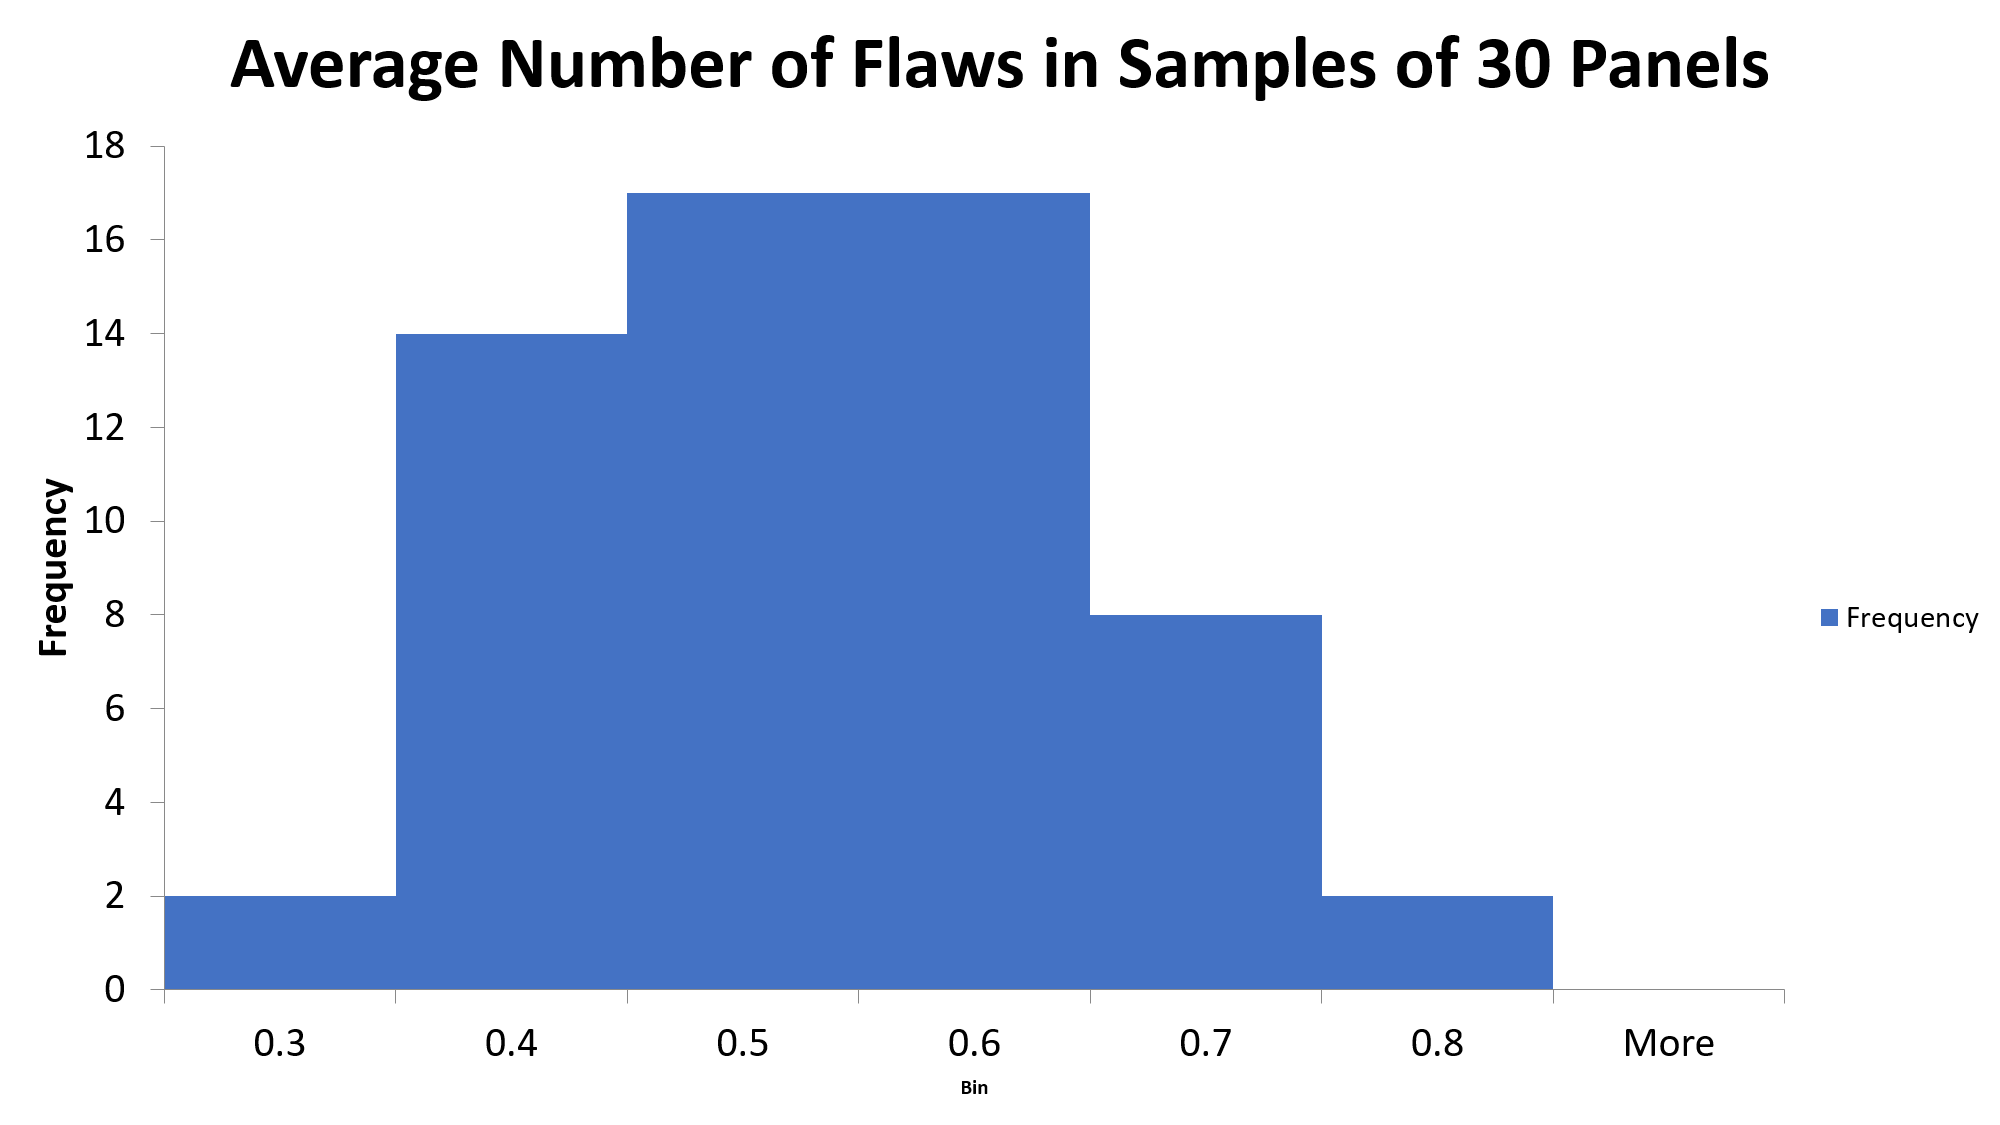
\includegraphics[width=\textwidth]{q5.png}
%  \caption{Average number of flaws in samples of 30 panels from 1800 plastic panels.}
%  \label{5a}
% \end{figure}

\end{document}
